\chapter{Régression Lasso}
\label{ch:ch4}
La méthode précédente produisant des variables d’importance relativement homogène, elle rend l’interprétation difficile. Afin de permettre aux radiologues d’identifier plus facilement les variables pertinentes ainsi que leur mode d’influence, nous avons exploré une approche alternative plus interprétable.

Nous avons ainsi réalisé une régression logistique en utilisant l’ensemble de nos paramètres numériques, identifiés par leur phase d'injection, comme variables explicatives, et la variable \texttt{Classe\_name} (valant 1 pour CHC et 0 pour CKC) comme variable cible. Pour l'entraînement du modèle, nous avons utilisé 80\,\% des données disponibles.

Les données de train et de test sont créées avec de l’échantillonnage stratifié pour avoir la même proportion de classe dans les deux ensembles,

La régression aboutit à une équation de la forme :
\[
\scriptstyle
Y = \beta X,\quad \text{avec } \beta = (\beta_1, \dots, \beta_{528}), \; X = (X_1, \dots, X_{528}),
\]
où les coefficients $\beta_j$ sont estimés par maximisation de la vraisemblance.

Afin de sélectionner uniquement les variables les plus pertinentes, nous avons appliqué une pénalisation de type \textit{Lasso} (L1). Cette méthode force certains coefficients $\beta_j$ à s’annuler, ne conservant que ceux dont l’impact est significatif sur la prédiction. Cela permet une meilleure interprétation du rôle de chaque variable dans la classification.

Nous avons ensuite tracé la courbe ROC du modèle (représentant le taux de vrais positifs en fonction du taux de faux positifs pour chaque seuil de classification). Le point optimal, situé le plus près du coin supérieur gauche du graphique, correspond à un seuil de classification de 0{,}21. À ce seuil, le modèle atteint une précision de 80\,\%, mais la sensibilité (c’est-à-dire la capacité du modèle à détecter correctement les cas positifs, ici les CKC) n’est que de 57\,\%.

\begin{figure}[H]
    \centering
    \includegraphics[width=0.4\textwidth]{img/roc.jpg}
    \caption{Figure: Courbe ROC}
\end{figure}


Cette faible sensibilité s’explique en grande partie par le déséquilibre entre les classes. C’est pourquoi nous nous intéressons également à la précision pondérée, qui atteint 72\,\% et prend en compte le déséquilibre des classes dans l’évaluation globale du modèle.

Une analyse du modèle donne comme variables prépondérantes les variables : 

\begin{table}[H]
    \centering
    \resizebox{\columnwidth}{!}{
    
    \begin{tabular}{|c|c|c|}
    \hline
    \textbf{Niveau de gris} & \textbf{Forme} & \textbf{Texture} \\
    \hline
    \texttt{original\_firstorder\_10Percentile} & \texttt{original\_shape\_Elongation} & \texttt{original\_gldm\_DependenceVariance}, \\
     & & \texttt{DependenceEntropy}, \\
     & & \texttt{LargeDependenceHighGrayLevelEmphasis} \\
    \hline
    \texttt{original\_firstorder\_Energy} & \texttt{original\_shape\_Sphericity} & \texttt{original\_glcm\_InverseVariance} \\
    \hline
    \texttt{original\_firstorder\_Skewness} & & \texttt{original\_glszm\_GrayNonUniformityNormalized}, \\
    & & \texttt{SmallAreaLowGrayLevelEmphasis} \\
    \hline
    \texttt{original\_firstorder\_TotalEnergy} & & \\
    \hline
    \end{tabular}}
    \caption{Tableau des variables radiomiques sélectionnées}
    \end{table}
Les variables les plus influentes sont celles avec un coefficient absolu le plus élevé, les négatives indiquant une augmentation de la probabilité d’être classé comme CKC et les positives d'être CHC.La distriubtion des coefficients est représentée dans la figure suivante.
\begin{figure}[H]
    \centering
    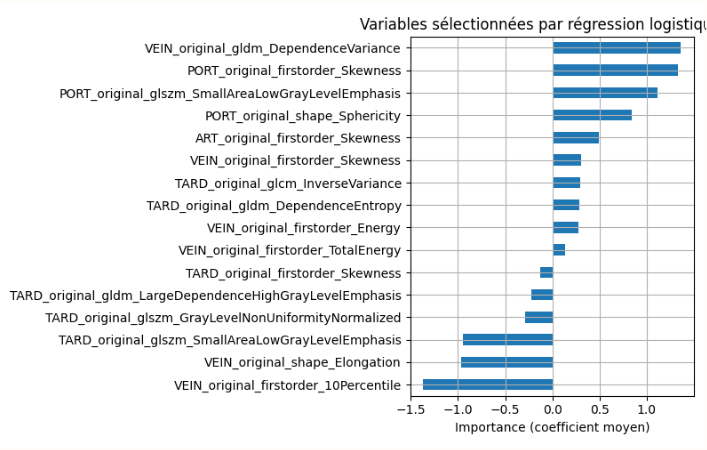
\includegraphics[width=0.5\textwidth]{img/variables.png}
    \caption{Influence des variables sélectionnées}
\end{figure}
